%Capa
\imprimircapa


%Folha de rosto sem número de página
\setcounter{page}{3}
\imprimirfolhaderosto*


% Ficha Catalográfica
\begin{fichacatalografica}
    \vspace*{\fill}
    \begin{center}
        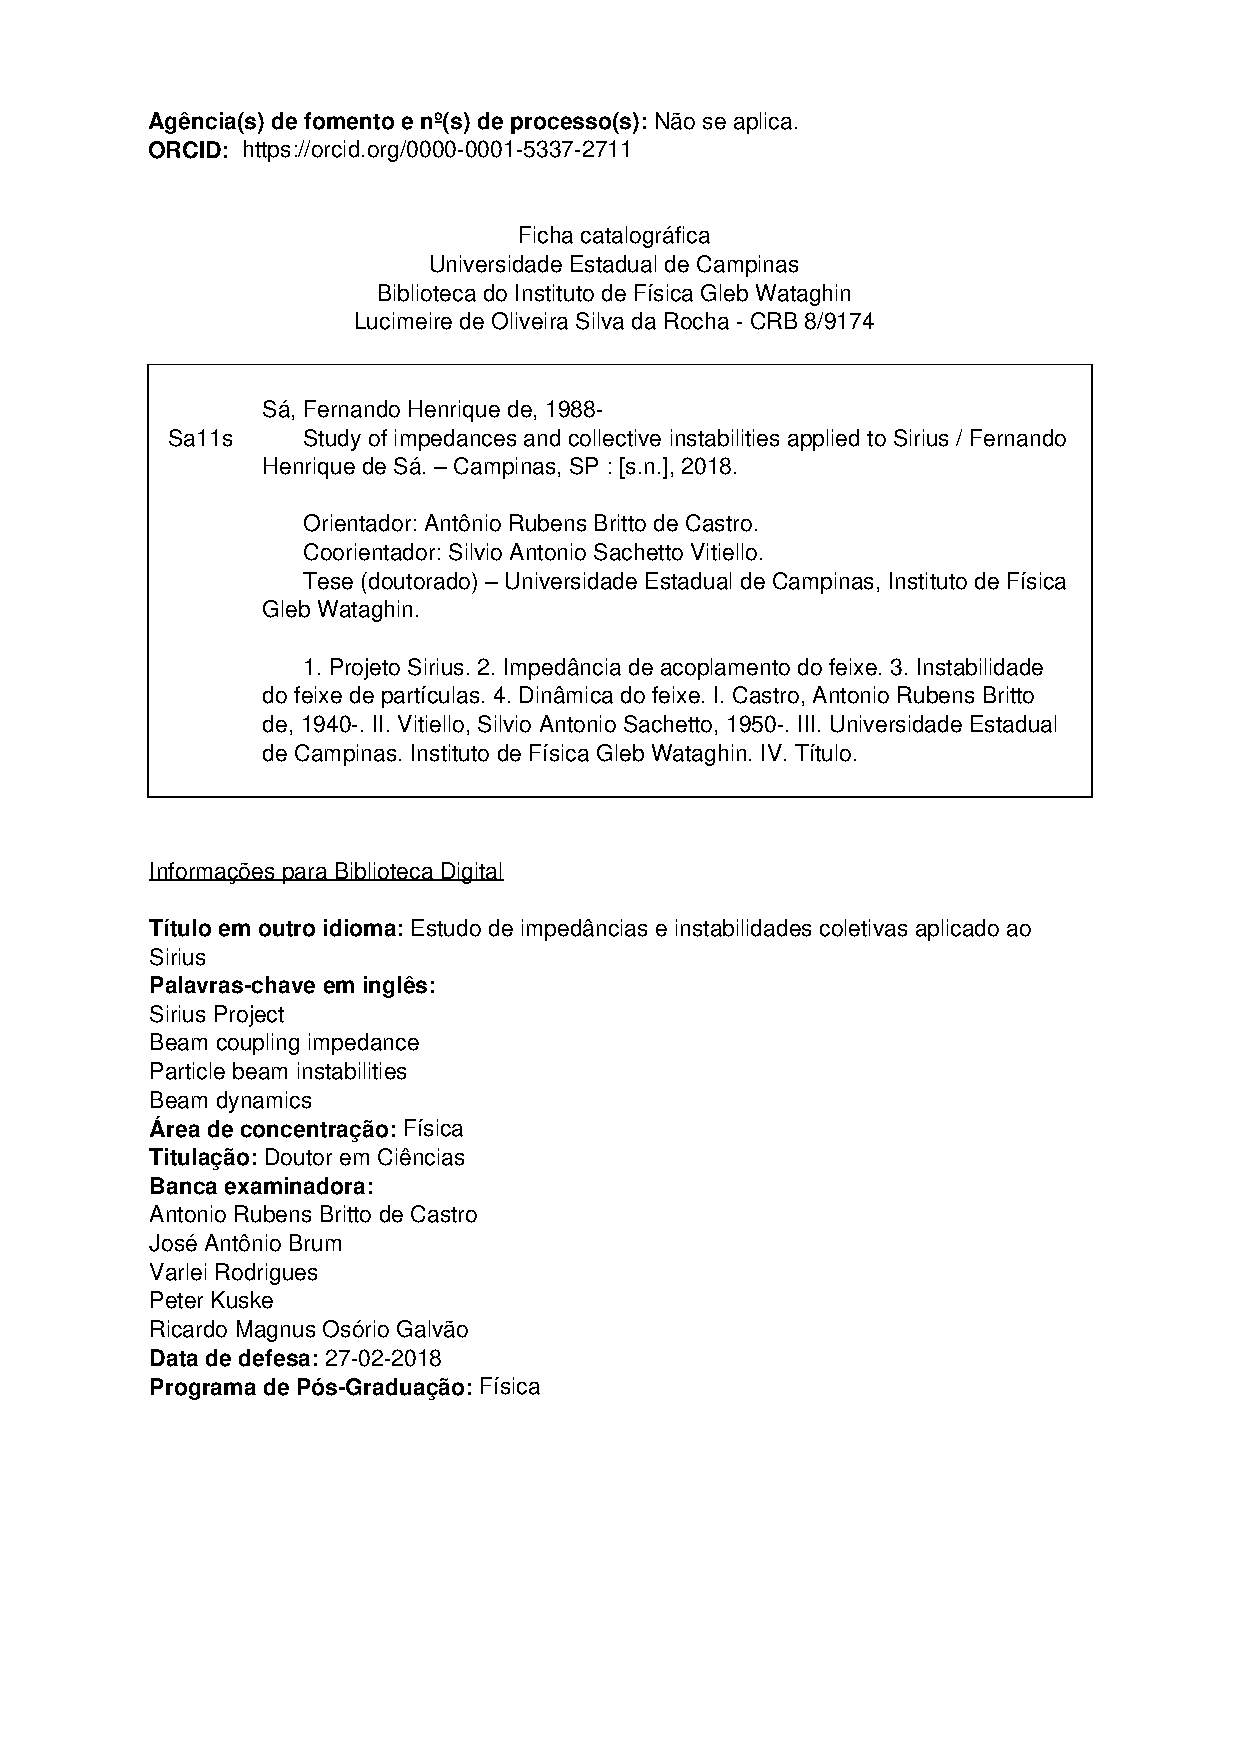
\includepdf{documents/ficha_catalografica.pdf}
    \end{center}
    \vspace*{\fill}
\end{fichacatalografica}

% Folha de aprovação
% Na versão final, tenho que excluir essas linhas e incluir o \includepdf
\vspace*{\fill}
\begin{center}
    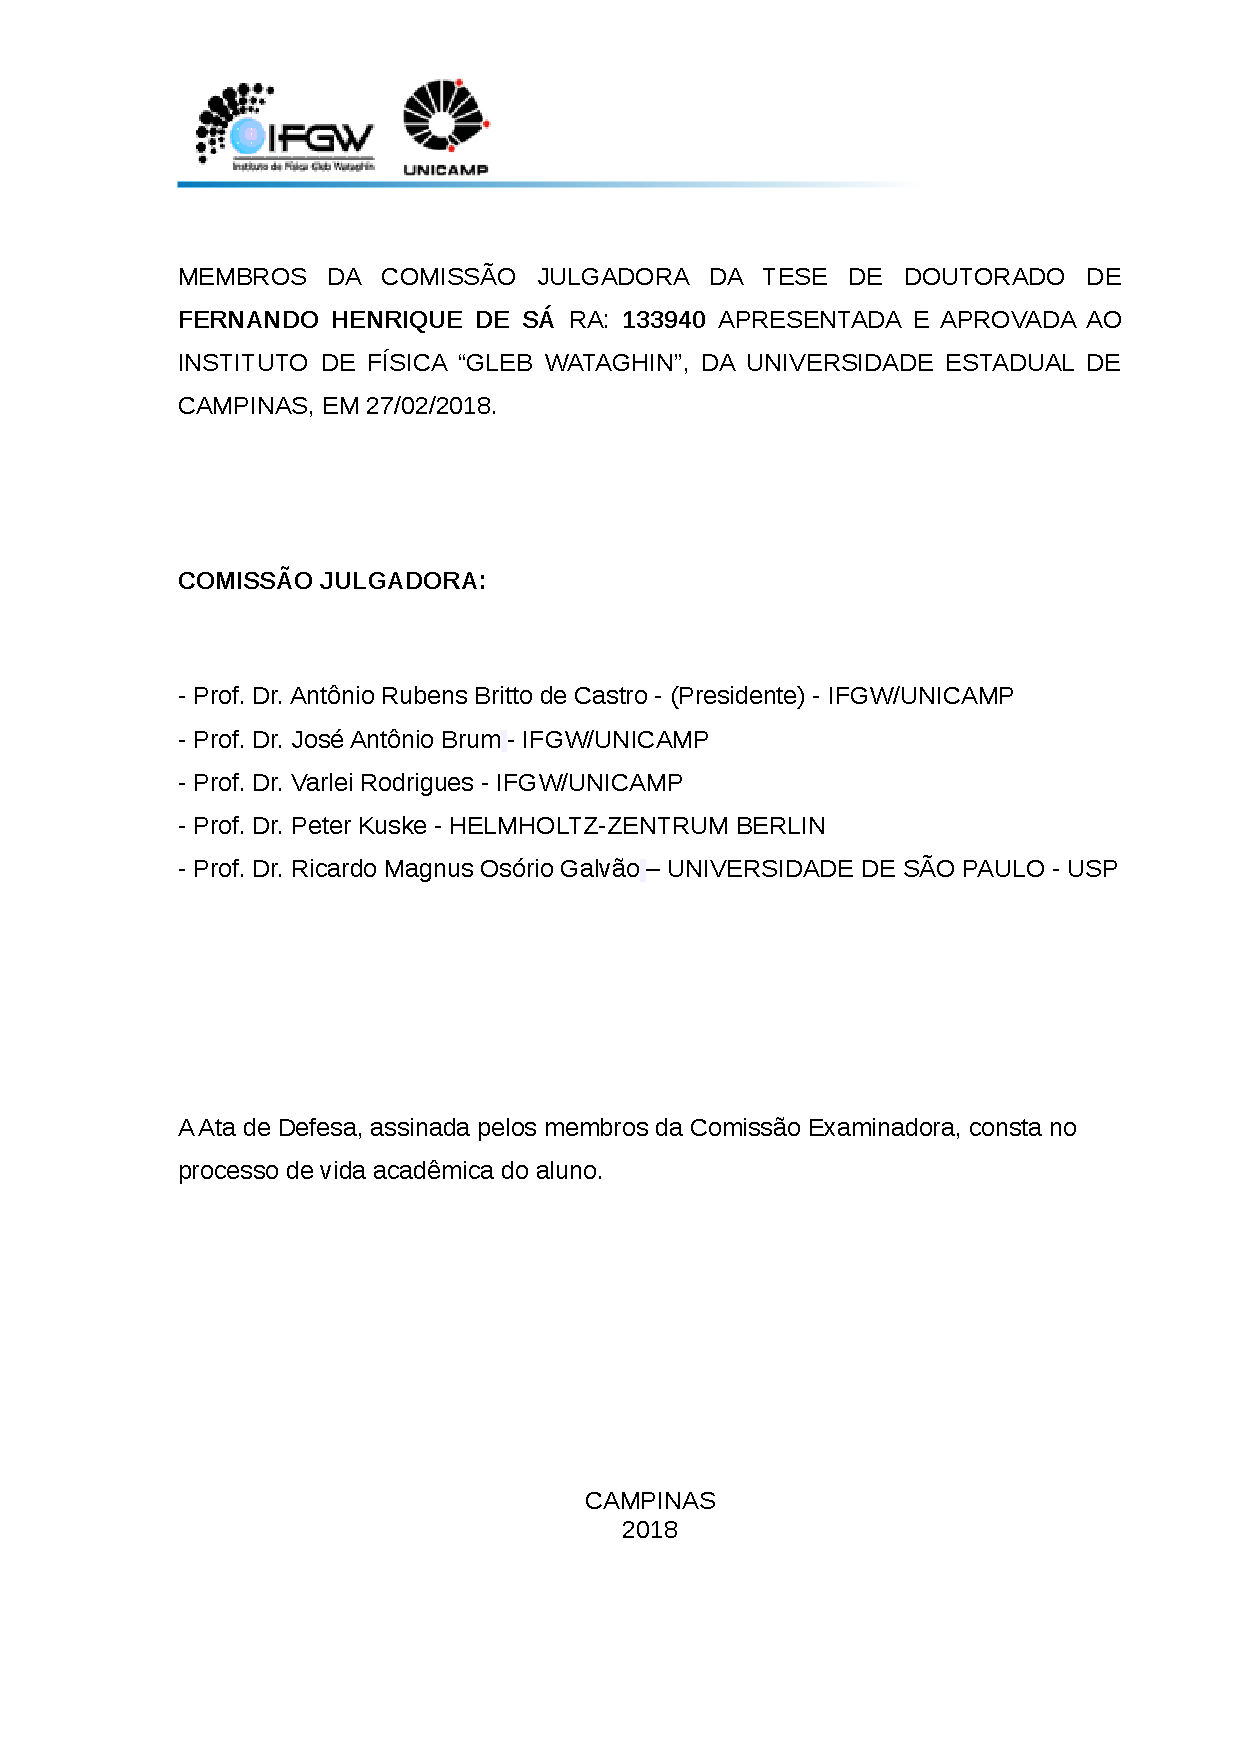
\includepdf[pagecommand={\thispagestyle{empty}}]{documents/capa_aprovacao.pdf}
\end{center}
\vspace*{\fill}
\cleardoublepage


% Dedicatória
\begin{dedicatoria}
    \vspace*{\fill}
    \centering
    \noindent
    \textit{À meus pais e avós.}
    \vspace*{\fill}
\end{dedicatoria}

% Agradecimentos
\begin{agradecimentos}
    Eu agradeço minha família por todo apoio durante esses anos, não só durante o doutorado como também em minha época de faculdade. Obrigado por entenderem e me apoiarem nos momentos que não pude passar com vocês, assim como nas vezes que meu corpo estava perto, mas minha cabeça distante. Se não fosse por tudo o que aprendi com vocês, a dedicação aos compromissos e ao trabalho e a aplicação em "fazer bem feito", eu provavelmente teria tomado o caminho mais cômodo e desistido do dourtorado. Além de serem meu alicerçe, vocês são um exemplo para mim.
    Também agradeço à Liu pelo incentivo em todos os momentos e por 
    Obrigado...
\end{agradecimentos}

% % Epígrafe
% \begin{epigrafe}
%     \vspace*{\fill}
%     \begin{flushright}
%         \textit{``O que você deixa para trás pode afetar o seu futuro.''\\
%         (Luana Nayara Pires Vilela)}
%     \end{flushright}
% \end{epigrafe}

% Resumos em português
\begin{resumo}
    Sirius is the new fourth generation light source that is being built in Campinas, Brazil, by the Brazilian Synchrotron Light Laboratory (LNLS). With a natural emittance of~\SI{250}{\pico\meter\radian}, extremely high--brightness synchrotron light will be generated by, at most,~\num{18}~insertion devices (IDs) installed in the straight sections of the storage ring and by~\num{20}~superbends (\SI{3.2}{\tesla}) present in the center of each achromat of the magnetic lattice. The standard vacuum chamber will be round, made of copper, with a radius of~\SI{12}{\milli\meter}, which is small compared to third generation light sources chambers, and the first IDs planned will be out of vacuum and will have a very reduced gap, with chambers as small as~\num{2.4}~and~\SI{3.0}{\milli\meter}, in most cases. Additionaly, vacuum pumping will be distributed, through the use of NEG coating at the inner surface of the chambers in the whole ring. All these factors intensify the impedance related effects of the machine, which can generate coherent oscillations, compromizing the quality of the light, cause total or partial beam loss and influence the equilibrium dynamics of the electrons. In this work some of the main components of the vacuum chamber were modelled and their wake fields were calculated with semi-analytical and numerical methods and added to the total impedance budget of the machine. With the application of this model to the first phase of operation, it was found that the beam will suffer from transverse coupled bunch resistive wall instability, making it necessary the installation of transverse bunch-by-bunch feedback systems in both planes. It was also predicted stability without feedback action provided that the ring operates with chromaticity larger than~\num{2.2} in both planes. The thresholds for intra-bunch instabilities are much above the nominal operation current and will not be a problem in any of the three planes and there will be no longitudinal coupled-bunch motion as long as the ring operates with superconducting RF cavities. The installation of a Landau cavity is planned for the phase two of operation, which will allow higher total current in the machine and even high single-bunch current in the middle of the train. Even though it was not done any calculations for these future operation conditions, the methods and codes developed in this work can be directly applied for those cases.
    % \vspace{\onelineskip}

    \noindent\textbf{Keywords}: Sirius Project; Impedance; Particle beam instabilities; Beam dynamics.
    \vspace{\fill}
\end{resumo}

% Resumo em Inglês
\begin{otherlanguage*}{brazil}
    \begin{center}{\ABNTEXchapterfont\huge Resumo}\end{center}
    Sirius é a nova fonte de luz síncrotron de quarta geração que está sendo construída em Campinas, Brasil, pelo Laboratório Nacional de Luz Síncrotron (LNLS). Com uma emitância natural de~\SI{250}{\pico\meter\radian}, radiação síncrotron de altíssimo brilho poderá ser gerada por até~\num{18}~dispositivos de inserção (DI) instalados nos trechos retos do anel de armazenamento e por~\si{20}~dipolos de alto campo (\SI{3.2}{\tesla}) presentes no centro de cada arco cromático da rede magnética. A câmara de vácuo padrão do anel será cilíndrica, feita de cobre e terá~\SI{12}{\milli\meter} de raio, que é um valor pequeno comparado às câmaras de fontes de luz síncrotron de terceira geração, e os primeiros DIs previstos serão fora do vácuo e terão uma abertura bastante reduzida, com câmaras de apenas~\num{2.4}~e~\SI{3.0}{\milli\meter}~de raio, na maioria dos casos. Adicionalmente, o sistema de vácuo do anel será distribuído, através da deposição de NEG na superfície interna das câmaras ao longo de todo o anel. Todos esses fatores intensificam os campos de arraste, ou impedâncias, da máquina, que podem gerar oscilações coerentes, deteriorando a qualidade da luz gerada, e causar perda total ou parcial do feixe, além de influenciar na dinâmica de equilíbrio dos elétrons. Neste trabalho alguns dos principais componentes da câmara de vácuo foram modelados e seus campos de arraste calculados por meios semi-analíticos e numéricos e adicionados ao modelo total de impedância do anel. Com a aplicação de tal modelo para a primeira fase de operação, constatou-se que o feixe será instável nos planos transverais devido a oscilações causadas por acoplamento entre pacotes gerados pela impedância de parede resistiva, tornando necessária a instalação de sistemas de retroalimentação pacote por pacote para manter a estabilidade. Também foi previsto que o feixe ficará estável se o anel for operado com uma cromaticidade nominal de \num{2.2} em ambos os planos transversais. Os limiares das instabilidades relacionadas a oscilações intra-pacote estão muito acima da corrente nominal de operação e não serão um problema. Não há previsão de instabilidades longitudinais de acoplamento entre pacotes, haja vista que a máquina operará com cavidades de RF supercondutoras. Na segunda fase de operação está prevista a instalação de uma cavidade Landau, que permitirá operação com corrente total mais alta, inclusive com pacotes bastante intensos no meio do trem. Apesar de não terem sido feitos cálculos para esse tipo de operação, os principais métodos e códigos desenvolvidos nesse trabalho podem ser diretamente usados para tal fim.

    \vspace{\onelineskip}
    \noindent\textbf{Palavras-chaves}: Projeto Sirius; Impedância; Instabilidades do feixe de partículas; Dinâmica do feixe.
    \vspace{\fill}
\end{otherlanguage*}
\cleardoublepage


% Lista de ilustrações
\pdfbookmark[0]{\listfigurename}{lof}
\listoffigures*
\cleardoublepage


% Lista de tabelas
\pdfbookmark[0]{\listtablename}{lot}
\listoftables*
\cleardoublepage

% Lista de Acronimos e Abreviações
% \renewcommand{\nomname}{Acronyms}
% \pdfbookmark[0]{\nomname}{las}
% \printnomenclature
\printglossaries
\cleardoublepage


% Sumário
\pdfbookmark[0]{\contentsname}{toc}
\tableofcontents*
\cleardoublepage
